\chapter{Results}

The Artefact that was created in Chapter \ref{ch3} could identify StyleGAN images with very high accuracy. The various results achieved in the development of the Artefact will be discussed and evaluated. The initial neural network accuracy will be discussed and example output from the artefact making the predictions will be demonstrated. The hyperparameter optimized neural network that acts as this project final model will be compared to the initial model and the model created by \cite{Wang} to demonstrate the large gains made to the model performance using optimization in constrained resources environment. 

\section{The First Neural Network}

The neural network created in Sprint 1 produced a detection accuracy of 61\% by just replacing StyleGAN generated and real human images with the Cat-vs-Dog images in the introduction to CNN's exercise. The accuracy achieved acted as a proof of concept. Using Hot and Cold learning techniques improved the model to a training accuracy of 81\%. When testing the improvements made in hot and cold learning the real accuracy that the model identifies StyleGAn images was 69\%, which means the model still cannot extract features from the images in the dataset but can generalize some features. The relatively high accuracy of the simplest implementation and the increase in accuracy when applying hot and cold learning shows how powerful CNN's can be in a world with increasing artificially generated images. Figure \ref{fig:reswrong} shows the self-created model implemented in the front-end artefact predicting on StyleGAN images and real human images from the FlickrFaces dataset. Although the model's prediction confidence is low, the prediction is advantageous compared to a random guess. A random guess and a neural network accuracy of 50\% can be seen as providing the same value. If a model predicts with only 50\% accuracy then code that mimics a coin flip prediction by random selection will provide the same results to the user. Therefore with the first neural network model starting with an accuracy higher than 60\% and the then reworked model providing an accuracy of 69\% was the value added by this project successful from the first iteration of the artefact development. Figure \ref{fig:reswrong} below shows the initial models deficiencies when identifying StyleGAN images.

\begin{figure}[H]%
\centering
\fbox{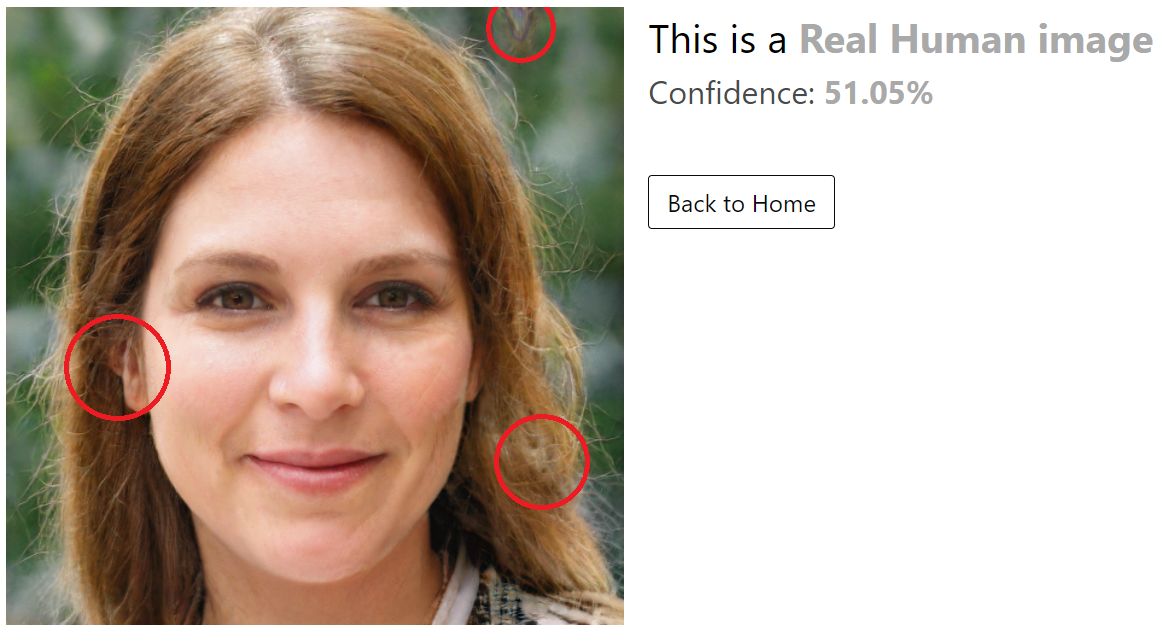
\includegraphics[width=0.95\textwidth]{img/fwrong.png}}%
\caption{Incorrect prediction from the initial model}%
\label{fig:reswrong}%
\end{figure}

Figure \ref{fig:reswrong}  and Table \ref{tabl:res1} shows the neural network that was created based on the activities in the 1st Sprint and concluded in the second sprint using hot and cold learning. The model correctly predicts most human images it receives but struggles with identifying StyleGAN images. What was obtained from this real image tending accuracy is that in the event of a StyleGAN prediction the user can be sure that the image has counter fitting properties, in this problem that would be StyleGAN artefact. That means that this model can be used in practice but only to a certain extent and cannot provide strong assurance. The results in Table \ref{tabl:res1} further illustrates the model's accuracy with real human images and its struggle with StyleGAN generated images.

\begin{table}[!htbp!]%
\caption{Real Images detected vs StyleGAN images detected in the initial model}
\label{tabl:res1}
\centering
\large
%\resizebox{0.60\textwidth}{!}{
\begin{tabular}{cccc}
\hline
Type of Image & & & Identification Accuracy  \\ 
\hline
StyleGAN & & & 68.00\% \\
Real Human & & & 77.20\% \\
\hline
\end{tabular}

\end{table} 

The misclassification of the initial model can partly be due to it not being optimized and therefore missing fine features in StyleGAN images. Some generalization occurred in this model and thus the results of the accuracy in SyleGAN misclassification echoed into the results of Real Human detection with high accuracy.

\section{The Optimized model}

The final model that was created in Sprint 3 improved in accuracy drastically. The model compared to the previous model is shown in Table below and a clear gain inaccuracy can be seen. The optimized model improved to such a high level of feature recognition in the StyleGAN data that the models prediction on StyleGAN2 generated images is similar to the First model created in the artefact developments prediction on StyleGAN1 images. Optuna greatly improved to model to such a high accuracy level in StyleGAN1 models that the model can contend with the model created by \cite{Wang} for the identification of CNN images. If using only StyleGAN1 images the model that was created for the artefact of this project is as effective as the model created by \cite{Wang}. The improvement that was made on the process for the model created in this project is the less restraining training and requirements for resources.

\begin{table}[!htbp!]%
\caption{Model comparison in terms of Accuracy and Confidence}
\label{tabl:res2}
\centering
\large
%\resizebox{0.60\textwidth}{!}{
\begin{tabular}{cccc}
\hline
Created Models & & Tested Accuracy  & Average Confidence\\ 
\hline
Cat-vs-Dog replacement & & 61.00\% & 57.00\%\\
Hot and Cold learning & & 69.00\% & 65,37\%\\
Hyperparameter Optimized & & 97,60\% & 96,98\%\\
\hline
\end{tabular}

\end{table} 


As shown in Table \ref{tab1:res2} implementing hyperparameter optimization on the StyleGAN identification problem improved the model to such a high accuracy that the model can be used in the industry, such as image verification services on dating websites. The higher confidence average that the optimized model produces on a single prediction is a important metric of the models overall performance. When a model receives an image and makes it's prediction the confidence metric that is also returned to the user in the front-end of the application will aid in a better identification "accuracy" that the model can provide. In the event of a miss classification the overall confidence level of the models prediction will be lower than the average confidence of the network. Therefore even in the event of a miss identification of a StyleGAN image, the user can reference the low confidence level and know that something regarding that image is not standard and a second evaluation might be necessary.

In Figure a random StyleGAN image and a real human image not contained in the FlickrFaces dataset is passed to the neural network model in the working complete artefact. The Optuna optimized model identifies the images correctly and illustrated its high confidence in its correct prediction. 

Optuna Miscalssifying

Improved classification neels

Optuna on StyleGAN2

Table of all network accuracies

Conclusion

